%==============================================================================
% Chapitre 54 - Les projectiles de chasse
%==============================================================================

\section{Introduction}

Les projectiles de chasse présentent une grande diversité de formes et de
conceptions.

Contrairement aux munitions militaires, leur objectif principal est
généralement de produire un effet terminal adapté au gibier recherché.

La déformation du projectile après impact constitue souvent un critère de
conception important.

\begin{aretenir}

Un projectile de chasse est généralement conçu pour transférer efficacement
son énergie à la cible.

\end{aretenir}

\section{Les objectifs recherchés}

Les concepteurs cherchent souvent à obtenir un compromis entre :

\begin{itemize}
    \item précision ;
    \item pénétration ;
    \item expansion ;
    \item conservation de masse ;
    \item sécurité.
\end{itemize}

Ces critères peuvent parfois être contradictoires.

\section{La balle blindée}

La balle blindée possède une chemise métallique entourant le noyau.

Bien qu'elle puisse être utilisée pour certaines applications spécifiques,
elle reste relativement peu employée à la chasse.

Sa déformation limitée réduit généralement le transfert d'énergie.

\section{La balle demi-blindée}

La balle demi-blindée constitue l'une des conceptions les plus répandues.

Une partie du noyau est laissée apparente à l'avant du projectile.

Cette configuration favorise l'expansion après impact.

\begin{figure}[htbp]
\centering

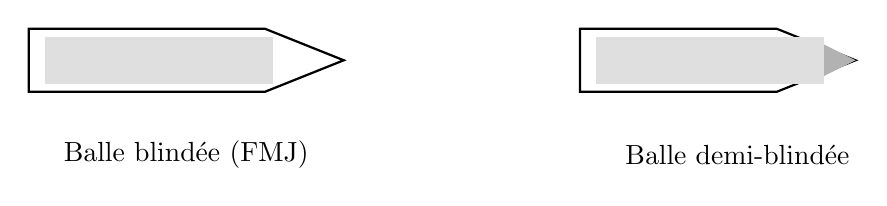
\begin{tikzpicture}[scale=1]

% FMJ
\draw[thick]
(0,0)
--
(0,0.8)
--
(3,0.8)
--
(4,0.4)
--
(3,0)
--
cycle;

\fill[gray!25]
(0.2,0.1)
rectangle
(3.1,0.7);

\node at (2,-0.8) {Balle blindée (FMJ)};

% Demi-blindée
\begin{scope}[xshift=7cm]

\draw[thick]
(0,0)
--
(0,0.8)
--
(2.5,0.8)
--
(3.5,0.4)
--
(2.5,0)
--
cycle;

\fill[gray!25]
(0.2,0.1)
rectangle
(3.1,0.7);

\fill[gray!60]
(3.1,0.2)
--
(3.5,0.4)
--
(3.1,0.6)
--
cycle;

\node at (2,-0.8) {Balle demi-blindée};

\end{scope}

\end{tikzpicture}

\caption{Comparaison simplifiée entre une balle blindée et une balle demi-blindée.}
\label{fig:fmj_demi_blindee}

\end{figure}

\section{Principe de l'expansion}

Lors de l'impact, la partie avant du projectile se déforme progressivement.

Cette déformation augmente généralement :

\begin{itemize}
    \item le diamètre apparent ;
    \item la surface de contact ;
    \item le transfert d'énergie.
\end{itemize}

\begin{figure}[htbp]
\centering

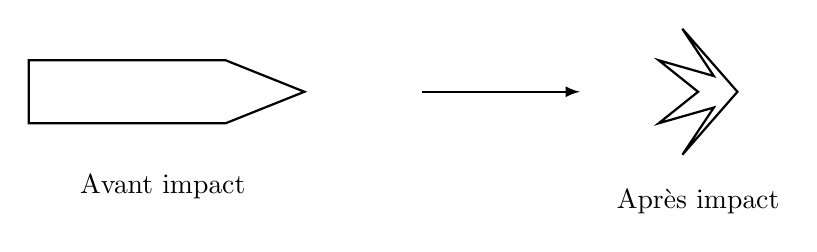
\begin{tikzpicture}[scale=1]

% Avant
\draw[thick]
(0,0)
--
(0,0.8)
--
(2.5,0.8)
--
(3.5,0.4)
--
(2.5,0)
--
cycle;

\node at (1.7,-0.8) {Avant impact};

% Flèche
\draw[-latex,thick]
(5,0.4)
--
(7,0.4);

% Après
\draw[thick]
(9,0.4)
--
(8.3,1.2)
--
(8.7,0.6)
--
(8,0.8)
--
(8.5,0.4)
--
(8,0)
--
(8.7,0.2)
--
(8.3,-0.4)
--
cycle;

\node at (8.5,-1.0) {Après impact};

\end{tikzpicture}

\caption{Principe simplifié de l'expansion d'une balle de chasse.}
\label{fig:expansion_balle}

\end{figure}

\section{La balle à pointe creuse}

La balle à pointe creuse comporte une cavité située à l'avant.

Cette cavité facilite l'ouverture du projectile lors de l'impact.

\begin{figure}[htbp]
\centering

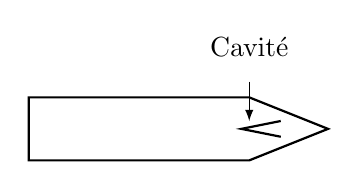
\begin{tikzpicture}[scale=1]

\draw[thick]
(0,0)
--
(0,0.8)
--
(2.8,0.8)
--
(3.8,0.4)
--
(2.8,0)
--
cycle;

% Cavité
\draw[thick]
(3.2,0.3)
--
(2.7,0.4)
--
(3.2,0.5);

\node[above] at (2.8,1.2)
{Cavité};

\draw[-latex]
(2.8,1.0)
--
(2.8,0.5);

\end{tikzpicture}

\caption{Coupe simplifiée d'une balle à pointe creuse.}
\label{fig:pointe_creuse}

\end{figure}

\section{La balle à pointe polymère}

Certaines conceptions modernes utilisent une pointe en matériau polymère.

Cette pointe améliore souvent :

\begin{itemize}
    \item l'aérodynamique ;
    \item la régularité de l'expansion ;
    \item la précision.
\end{itemize}

\section{Les projectiles monolithiques}

Les projectiles monolithiques sont réalisés dans un seul matériau.

Ils sont souvent usinés à partir d'un alliage métallique.

\section{Conservation de masse}

Lors de l'impact, certains projectiles peuvent perdre une partie de leur
masse.

D'autres sont conçus pour conserver une proportion importante de leur masse
initiale.

Cette caractéristique influence directement la pénétration.

\section{Expansion contrôlée}

Les projectiles modernes cherchent souvent à limiter les comportements
imprévisibles.

L'expansion contrôlée vise à obtenir une déformation régulière et
reproductible.

\section{Pénétration}

Une pénétration suffisante demeure indispensable.

Un projectile qui s'expanse trop rapidement risque de ne pas atteindre les
organes recherchés.

\section{Compromis expansion-pénétration}

L'expansion et la pénétration constituent souvent deux objectifs opposés.

Une expansion importante tend à augmenter le transfert d'énergie mais peut
réduire la profondeur de pénétration.

\begin{figure}[htbp]
\centering

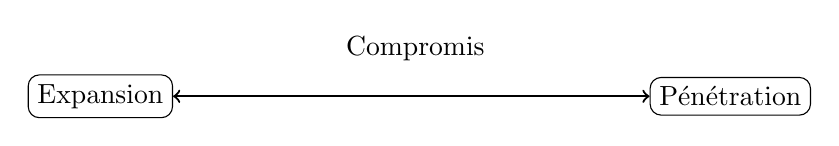
\begin{tikzpicture}[scale=1]

\node[draw,rounded corners]
(E)
at (0,0)
{Expansion};

\node[draw,rounded corners]
(P)
at (8,0)
{Pénétration};

\draw[<->,thick]
(E)
--
(P);

\node
at (4,0.6)
{Compromis};

\end{tikzpicture}

\caption{L'expansion et la pénétration constituent souvent des objectifs contradictoires.}
\label{fig:compromis_expansion_penetration}

\end{figure}

\section{Influence de la vitesse}

Le comportement terminal dépend fortement de la vitesse d'impact.

Un même projectile peut présenter des résultats différents selon :

\begin{itemize}
    \item la distance ;
    \item la vitesse résiduelle ;
    \item la nature de la cible.
\end{itemize}

\section{Le choix du projectile}

Le choix dépend notamment :

\begin{itemize}
    \item du gibier ;
    \item de la distance de tir ;
    \item du calibre ;
    \item de la réglementation.
\end{itemize}

\section{Évolution récente}

Les progrès des matériaux et des procédés de fabrication ont permis le
développement de projectiles de plus en plus spécialisés.

Les performances obtenues aujourd'hui étaient difficilement envisageables il y
a quelques décennies.

\section{Vers les cartouches de chasse}

Le projectile ne constitue qu'un élément de la munition.

Le chapitre suivant examinera plus en détail la structure complète des
cartouches de chasse modernes.

\begin{figure}[htbp]
\centering

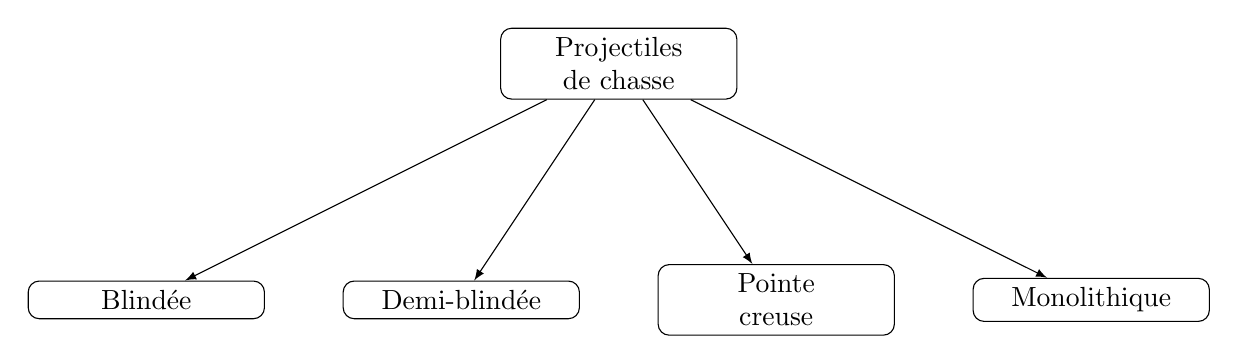
\begin{tikzpicture}[
every node/.style={
draw,
rounded corners,
align=center,
minimum width=3cm
}
]

\node (P) at (0,0) {Projectiles\\de chasse};

\node (F) at (-6,-3) {Blindée};
\node (D) at (-2,-3) {Demi-blindée};
\node (C) at (2,-3) {Pointe\\creuse};
\node (M) at (6,-3) {Monolithique};

\draw[-latex] (P) -- (F);
\draw[-latex] (P) -- (D);
\draw[-latex] (P) -- (C);
\draw[-latex] (P) -- (M);

\end{tikzpicture}

\caption{Principales familles de projectiles de chasse modernes.}
\label{fig:familles_projectiles_chasse}

\end{figure}

\section{À retenir}

\begin{aretenir}

\begin{itemize}
    \item Les projectiles de chasse sont conçus pour produire un effet terminal
          adapté.
    \item La balle demi-blindée reste très répandue.
    \item L'expansion contrôlée constitue un objectif majeur.
    \item La pénétration et l'expansion doivent être équilibrées.
    \item Les conceptions modernes utilisent des matériaux et géométries
          variés.
\end{itemize}

\end{aretenir}
